% !TeX root = ..\main.tex
% Chapter 4

\chapter{实验及结果分析}

为验证本系统在古诗生成、评价和优化方面的有效性,本文设计开展了相关实验,利用已有古诗数据集来检验系统性能,结合自动度量方法对比了ERNIE-4.0和DeepSeek-R1两种模型产出的结果。

\section{基于白话文的古诗生成实验}

参考相关工作中评估模型表现的方法,给定一个质量获得认可的古诗,将评估模型的输出古诗与这一古诗进行对比,利用BLEU和ROUGE计算指标分数\upcite{chenPolishingModelMachineGenerated2024}。在这一思路下,原古诗的质量应当足够好,以确保指标分数能够反映被评估输出的质量;且模型的输入要与原古诗的内容十分相关,以确保指标分数能够反映模型的生成能力。

为此,本文选择《唐诗三百首》中的名篇作为古诗原文,选择相应的白话文翻译作为文本输入。《唐诗三百首》是清代蘅塘退士孙洙编选的唐诗选集,问世不久便闻名遐迩,成为唐诗入门读物的首选,其中收录的唐诗均为名篇佳作。原书中除了律诗、绝句外,还收录有乐府、古体诗等形式多变的体裁,故不便于评估,本文仅选择律诗和绝句两种体裁的古诗进行测试,各体裁作品及数目见表~\ref{tab:test_generation_data}。此外,相应的白话文翻译源自古诗文网\upcite{Gushiwenwang}。

\begin{table}[ht]
    \centering
    \caption{《唐诗三百首》测试数据集}
    \label{tab:test_generation_data}
    \begin{tabular}{|c|c|}
      \hline
       \bf{体裁}& \bf{数量} \\
      \hline
      七言律诗& 51\\
      \hline
       七言绝句& 50\\
      \hline
       五言律诗& 80\\
      \hline
       五言绝句& 29\\
      \hline
       合计& 210\\
      \hline
    \end{tabular}
  \end{table}

测试发现,ERNIE-4.0和DeepSeek-R1两种模型的输出均与参考古诗有极高的覆盖度,因而在BLEU和ROUGE指标上均有很高的得分,明显区别于以往工作中的结果(如\verb|BLEU-1|=0.168, \verb|BLEU-2|=0.002\upcite{chenPolishingModelMachineGenerated2024}),属于异常情况。作为大模型,两种模型的训练数据均包含了大量的古诗数据,尤其是对《唐诗三百首》这样的名篇,因而本实验并不能做到训练集与测试集的独立,并不具备验证效果。
测试统计结果见表~\ref{tab:test_generation_tssbs_dsr1}和表~\ref{tab:test_generation_tssbs_ernie4}。


\begin{table}[ht]
  \centering
  \caption{白话文古诗生成实验结果(DeepSeek-R1)}
  \label{tab:test_generation_tssbs_dsr1}
  \begin{tabular}{cccccc}
      \toprule
      & \multicolumn{2}{c}{BLEU} & \multicolumn{3}{c}{ROUGE} \\
      \cmidrule(r){2-3} \cmidrule(l){4-6}
      & BL-1& BL-2& R-1& R-2& R-L\\
      \midrule
      七言律诗& 0.583599&\bf{0.432841}&\bf{0.557353}&\bf{0.349461}&0.527267\\
      七言绝句&0.559833&0.415325&0.562665&0.344502&0.540417\\
      五言律诗&\bf{0.597726}&0.432494&0.549401&0.337500&\bf{0.545573}\\
      五言绝句&0.523605&0.332445&0.495130&0.245845&0.471983\\
      \cmidrule{2-6} %添加2-4列的中线
      平均&0.575037&0.414674&0.546996&0.329415&0.529737\\
      \bottomrule
  \end{tabular}
\end{table}

\begin{table}[ht]
  \centering
  \caption{白话文古诗生成实验结果(ERNIE-4.0)}
  \label{tab:test_generation_tssbs_ernie4}
  \begin{tabular}{cccccc}
      \toprule
      & \multicolumn{2}{c}{BLEU} & \multicolumn{3}{c}{ROUGE} \\
      \cmidrule(r){2-3} \cmidrule(l){4-6}
      & BL-1& BL-2& R-1& R-2& R-L\\
      \midrule
      七言律诗&0.765951&0.671162&0.770484&0.609392&0.743464\\
      七言绝句&0.798136&0.702556&0.808346&0.649742&0.764375\\
      五言律诗&0.691980&0.533006&0.670557&0.445450&0.646720\\
      五言绝句&\bf{0.839312}&\bf{0.764698}&\bf{0.834125}&\bf{0.726052}&\bf{0.812500}\\
      \cmidrule{2-6} %添加2-4列的中线
      平均&0.767420&0.658670&0.765072&0.596372&0.734993\\
      \bottomrule
  \end{tabular}
\end{table}


\section{评分功能实验} \label{sec:experiment_scoring}

为了检验系统评分功能的有效性,本文尝试收集具有质量差异的古诗分组,通过先验的质量分层来验证系统评分的合理性。此外,也将使用BLEU等自动度量方法,检验这些自动度量方法的有效性。

选择第六届“诗词中国”传统诗词创作大赛\upcite{sczg}的公开获奖作品为测试集,测试系统评分功能的有效性和可信度。该大赛的评审专家均为古诗词领域的专家,且其评分标准公开透明,因而可以作为测试系统评分功能的参考。该比赛设有不同的作品体裁和比赛组别,而本文主要专注于格律要求较严格的律诗、绝句等体裁,因此为便于测试,只选取其中的律诗与绝句作品进行。% 测试结果见表~\ref{tab:test_scoring_prized_dsr1_detail}(系统评分)、表~\ref{tab:test_scoring_prized_dsr1_1}(BLEU和ROUGE)和表~\ref{tab:test_scoring_prized_dsr1_2}(Similarity和Distinct)。

测试发现,不同奖项组之间的评分存在差异但并不显著,而且在许多维度上优秀奖的得分最高,考虑是因为各奖项样本数量分布不均,噪声干扰较大,结论难有普适性。因此,将一、二、三等奖的作品进行合并,形成数目为28的样本组“一二三等奖”,再将其与优秀奖的平均得分进行比较,发现尽管差异仍然不算显著,但在各个维度上的比较结果都与真实的结果一致,即“一二三等奖”中古诗的的质量要好于“优秀奖”(见表~\ref{tab:test_scoring_prized_dsr1_detail})。

\begin{table}[ht]
  \centering
  \caption{获奖作品的评分实验(系统评分)}
  \label{tab:test_scoring_prized_dsr1_detail}
  \begin{tabular}{cccccccc}
      \toprule
      &格律规范& 意象意境& 主题思想& 语言锤炼&创新性& 总分&样本\\
      \midrule
      一等奖	&	\textbf{0.800} &	0.833 &	0.825 &	0.800 &	\textbf{0.850} &	0.820 &	2	\\
      二等奖	&	0.696 	&	0.767 	&	0.830 	&	0.800 	&	0.800 	&	0.770 	&	8	\\
      三等奖	&	0.793 	&	\textbf{0.836} 	&	\textbf{0.846} 	&	\textbf{0.828} 	&	0.825 	&	\textbf{0.825} 	&	18	\\
      \cmidrule{2-7} %添加2-4列的中线
      一二三	&	\textbf{0.768} 	&	\textbf{0.818} 	&	\textbf{0.839} 	&	\textbf{0.818} 	&	\textbf{0.821} 	&	\textbf{0.810} 	&	28	\\
      优秀奖	&	0.762 	&	0.805 	&	0.824 	&	0.798 	&	0.797 	&	0.796 	&	91	\\
      \cmidrule{2-7} %添加2-4列的中线
      平均	&	0.763 	&	0.808 	&	0.828 	&	0.802 	&	0.802 	&	0.800 	&	119	\\
      \bottomrule
  \end{tabular}
\end{table}

在自动度量方面,BLEU与ROUGE的比较结果与系统评分的结果类似,在“一二三等奖”内部的比较结果有波动,但对“一二三等奖”和“优秀奖”之间的比较结果一致且正确(见表~\ref{tab:test_scoring_prized_dsr1_1}),说明二者作为古诗生成领域使用最广泛的自动度量指标,具有一定的有效性。对Similarity和Distinct,二者“一二三等奖”内部的比较结果一致且正确,而且Similarity在三种不同奖项之间的得分差异相对显著,但“一二三等奖”与“优秀奖”的比较结果却与正确结果相反,除了\verb|Distinct-1|这一个指标,说明二者在古诗质量评估的有效性有待进一步验证(见表~\ref{tab:test_scoring_prized_dsr1_2})

\begin{table}[ht]
  \centering
  \caption{获奖作品的评分实验(BLEU+ROUGE)}
  \label{tab:test_scoring_prized_dsr1_1}
  \begin{tabular}{cccccc}
      \toprule
      &  \multicolumn{2}{c}{BLEU} & \multicolumn{3}{c}{ROUGE}\\
      \cmidrule(r){2-3} \cmidrule(l){4-6}
       & BL-1& BL-2& R-1& R-2& R-L\\
      \midrule
      一等奖	&	\textbf{0.968750} 	&	0.678427 	&	0.096657 	&	0.001543 	&	0.134217 	\\
      二等奖	&	0.953125 	&	\textbf{0.805106} 	&	0.108463 	&	\textbf{0.004658} 	&	0.142648 	\\
      三等奖	&	0.938999 	&	0.788950 	&	\textbf{0.119148} 	&	0.004140 	&	\textbf{0.149292} 	\\
      \cmidrule{2-6} %添加2-4列的中线
      一二三	&	\textbf{0.945848} 	&	\textbf{0.781568} 	&	\textbf{0.113968} 	&	\textbf{0.004003} 	&	\textbf{0.145957} 	\\
      优秀奖	&	0.934612 	&	0.749390 	&	0.107799 	&	0.003346 	&	0.143840 	\\
      \cmidrule{2-6} %添加2-4列的中线
      平均	&	0.937247 	&	0.756938 	&	0.109246 	&	0.003500 	&	0.144337 	\\
      \bottomrule
  \end{tabular}
\end{table}

\begin{table}[ht]
  \centering
  \caption{获奖作品的评分实验(Similarity+Distinct)}
  \label{tab:test_scoring_prized_dsr1_2}
  \begin{tabular}{ccccc}
      \toprule
      & \multicolumn{2}{c}{Similarity} & \multicolumn{2}{c}{Distinct}\\
      \cmidrule(r){2-3} \cmidrule(l){4-5} 
      & S-Intra& S-Inter& D-1& D-2\\
      \midrule
      一等奖&	\bf{0.675846} 	&	\bf{0.722989} 	&	\bf{0.906250} 	&	\bf{1.000000} 	\\
      二等奖&	0.660678 	&	0.697867 	&	0.890625 	&	\bf{1.000000} \\
      三等奖&	0.658698 	&	0.688951 	&	0.879656 	&	0.998677 	\\
      \cmidrule{2-5} %添加2-4列的中线
      一二三&	0.661024 	&	0.694880 	&	\bf{0.885342} 	&	0.999165 \\
      优秀奖&	\bf{0.670973} 	&	\bf{0.696803} 	&	0.879247 	&	\bf{0.999832} 	\\
      
      \cmidrule{2-5} %添加2-4列的中线
      平均&	0.668639 	&	0.696352 	&	0.880676 	&	0.999675 	\\

      \bottomrule
  \end{tabular}
\end{table}

为进一步检验评分功能及各自动度量方法的有效性,本文扩大测试古诗范围。由于“诗词中国”传统诗词创作大赛的往届获奖作品并不公开,因而无法获取更多带有可信等级标签的古诗作品。由此,本文纳入经典唐诗和打油诗两类数据集,退而求其次,尝试用世人公认的名篇作品与和质量明显较差的打油诗作为测试数据集。其中,从古诗文网挑选20首打油诗(见本节末图~\ref{fig:data_doggerel}),结合《唐诗三百首》中的共98首律诗(包括五言和七言),与来自比赛的获奖作品“一二三等奖”与“优秀奖”一同合并作为测试集。

测试发现,系统对四个作品集的评分具有稳定的差异,且每个维度上得分的大小关系与真实结果完全一致(见表~\ref{tab:test_scoring_all_dsr1_detail})。值得一提的是,在使用了新的评分体系后,系统对打油诗的评分降低到了$0.48$,显著低于之前工作的评分$0.67$,而获奖作品与经典唐诗的得分也有显著差距,有力地证明了新评分体系的有效性。

\begin{table}[ht]
  \centering
  \caption{纳入唐诗和打油诗的评分实验(系统评分)}
  \label{tab:test_scoring_all_dsr1_detail}
  \begin{tabular}{cccccccc}
      \toprule
      &格律规范& 意象意境& 主题思想& 语言锤炼&创新性& 总分& 样本\\
      \midrule
      唐诗	&	\bf{0.932} 	&	\bf{0.934} 	&	\bf{0.931} 	&	\bf{0.930} 	&	\bf{0.853} 	&	\bf{0.924} 	&	98	\\
      一二三	&	0.768 	&	0.818 	&	0.839 	&	0.818 	&	0.821 	&	0.810 	&	28	\\
      优秀奖	&	0.762 	&	0.805 	&	0.824 	&	0.798 	&	0.797 	&	0.796 	&	91	\\
      打油诗	&	0.328 	&	0.490 	&	0.615 	&	0.470 	&	0.585 	&	0.481 	&	20	\\									
      \bottomrule
  \end{tabular}
\end{table}

在自动度量方面,BLEU与ROUGE均能较好地反映古诗质量,除BLEU-1外的其他指标均与真实比较结果保持一致,进一步验证了二者在古诗质量评估方面的有效性。对BLEU-1,获奖作品的平均得分要高于经典唐诗,说明基于$1$-gram覆盖度的精度计算方法仍存在局限。(见表~\ref{tab:test_scoring_all_dsr1_1})。

\begin{table}[ht]
  \centering
  \caption{纳入唐诗和打油诗的评分实验(BLEU+ROUGE)}
  \label{tab:test_scoring_all_dsr1_1}
  \begin{tabular}{cccccc}
      \toprule
      &  \multicolumn{2}{c}{BLEU} & \multicolumn{3}{c}{ROUGE}\\
      \cmidrule(r){2-3} \cmidrule(l){4-6}
      & BL-1& BL-2& R-1& R-2& R-L\\
      \midrule
      唐诗	&	0.905665 	&	\bf{0.792163} 	&	\bf{0.125864} 	&	\bf{0.005379} 	&	\bf{0.157440} 	\\
      一二三	&	\bf{0.945848} 	&	0.781568 	&	0.113968 	&	0.004003 	&	0.145957 	\\
      优秀奖	&	0.934612 	&	0.749390 	&	0.107799 	&	0.003346 	&	0.143840 	\\
      打油诗	&	0.893658 	&	0.726545 	&	0.095770 	&	0.003127 	&	0.137659 	\\
      \bottomrule
  \end{tabular}
\end{table}

\begin{table}[ht]
  \centering
  \caption{纳入唐诗和打油诗的评分实验(Similarity+Distinct)}
  \label{tab:test_scoring_all_dsr1_2}
  \begin{tabular}{ccccc}
      \toprule
      & \multicolumn{2}{c}{Similarity} & \multicolumn{2}{c}{Distinct}\\
      \cmidrule(r){2-3} \cmidrule(l){4-5} 
      & S-Intra& S-Inter& D-1& D-2\\
      \midrule
      唐诗	&	0.678716 	&	0.693137 	&	0.854964 	&	0.998430 	\\
      一二三	&	0.661024 	&	0.694880 	&	\bf{0.885342} 	&	0.999165 	\\
      优秀奖	&	0.670973 	&	0.696803 	&	0.879247 	&	\bf{0.999832} 	\\
      打油诗	&	\bf{0.698042} 	&	\bf{0.738067} 	&	0.760565 	&	0.972817 	\\

      \bottomrule
  \end{tabular}
\end{table}

对Similarity,其两个指标\verb|S-Intra|和\verb|S-Inter|的对比结果与真实的质量等级并不一致,其中后者的结果甚至完全相反(见表~\ref{tab:test_scoring_all_dsr1_2})。Similarity使用词向量模型来考察古诗内前后文的语义相似度,分别计算古诗中前后句子间和不同联之间的相似度均值,体现的是古诗的语义连贯性,但这里的语义是词向量模型从数据集中学习到的,是对古诗的真实语义的近似,而非其自身。进一步测试发现,对打油诗“{\kaishu 天气好热燥,花开正繁闹。人静自然凉,心宽无烦恼}”和名篇《登鹳雀楼》“{\kaishu 白日依山尽,黄河入海流。欲穷千里目,更上一层楼}”,\verb|S-Intra|的结果分别为$\text{S-Intra}=0.671893$和$\text{S-Intra}=0.727715$,而\verb|S-Inter|的结果分别为$\text{S-Inter}=0.727715$和$\text{S-Inter}=0.659923$。这说明后者的联内上下句的语义相似度要高于前者(即“{\kaishu 白日依山尽}”和“{\kaishu 黄河入海流}”、“{\kaishu 欲穷千里目}”和“{\kaishu 更上一层楼}”),但联间的语义相似度要低于前者(即“{\kaishu 白日依山尽,黄河入海流}”和“{\kaishu 欲穷千里目,更上一层楼}”)

考虑指标自身的设计,对古诗作品而言,联内上下句往往因“对仗”而在形式、语法上有相似之处,因而\verb|S-Intra|能够反映一定的语义连贯性,尽管比较结果不显著,仍能作为评估古诗质量的参考。但对\verb|S-Inter|,联间的上下句往往在形式、语法上有差异,一般作品的不同联之间会切换意象或主题,或是表达不同的情感,因而语义差异较大,相反,若全诗通篇使用同一意象或主题,或是表达同一种情感,反而会因意象单薄而质量欠佳,所以这一指标的合理性欠佳。

但同时也需要考虑词向量模型的影响。在过往研究中使用的词向量,是在Bert模型基础上通过添加额外的向量得到的(额外的向量包含情感、声调、节奏、位置等),且词向量表示均是重新训练,并在在计算Similarity时直接使用的\upcite{chenPolishingModelMachineGenerated2024,dengIterativePolishingFramework2020}。因此,本文使用的词向量模型Bert-CCPoem可能并不适用于这类下游任务,仍有待进一步研究。

% 基于词向量的语义相似度计算方法具有相当的局限性,其或许受限于形式上诗句用词的对照,会因语法结构的对称而误判为高质量的语义相关,从而难以反映更深层次的语义连贯性。

对Distinct,\verb|D-1|和\verb|D-2|分别表示古诗中$1$-gram和$2$-gram的多样性,一定程度上反映了古诗在用词方面的创新性。测试发现,打油诗的\verb|D-1|和\verb|D-2|均低于经典唐诗和获奖作品,但得分最高者却分别为“一二三等奖”和“优秀奖”,这说明现代人的古诗作品或许在用词上会追求多样性。但与此同时,这也说明Distinct的计算方法并不能独立地反映古诗质量。

\begin{tcolorbox}[
  colback=white, % 背景透明
  colframe=black, 
  boxrule=1pt,        % 设置边框宽度
  arc=0mm             % 取消圆角
  ]
  \kaishu 
  \begin{enumerate}
      \item 盆中有山有水,心里无城无府。独行不怕天黑,苟活休论贫富。
      \item 天气好热燥,花开正繁闹。人静自然凉,心宽无烦恼。
      \item 一轮红日上青天,未到西河不罢川。今朝又见千年日,千年一叹又江山。
      \item 呼风唤雨太平常,摘颗星星袋里藏。家住东方不老岛,海山仙国是吾乡偶尔天上去逛逛,吓得日月不放光。一口喝尽银河水,惊倒王母喊玉皇。如来问我何神圣,我道人间打油郎。
      \item 一杯二杯三四杯,五杯六杯七八杯。九杯十杯开开胃,百杯干杯入微微。喝到万杯方半醉,亿杯兆杯不是吹。饮尽天上人间酒,始觉眼前牛在飞。骑牛飞到月宫去,嫦娥姐姐来作陪。
      \item 吾手写吾心,诗词随口吟。从不标牌体,管它古与新。
      \item 嫦娥仙子爱出楼,惹得人间看不休。雪白兔儿天上遛,银色蛤蟆水里游。
      \item 江上一笼统,井上黑窟窿。黄狗身上白,白狗身上肿。
      \item 一浪一浪又一浪,浪浪撞在石头上;明知前浪折了腰,后浪还要跟着上。
      \item 时光催人老,不比不知晓。少年在眼前,才觉白发早。
      \item 君自遥远故乡来,却说故乡在眼前。来日村口茶飘香,何不饮后才向前。他日回到故乡去,可知茶味如从前?
      \item 东也湖,西也湖,洪城上下古月胡;南长清,北长清,大街小巷胡长清。
      \item 一言一行一约定,一生一世一爱情。一轮一回一醉梦,一分一秒一旧心。纷纷扬扬雨,思思念念泪。凄凄凉凉夜,甜甜酸酸味。
      \item 海枯石烂荡耳边,沧海桑田共誓言。风风雨雨同路走,携手白头哪一站。
      \item 风风雨雨同路走,偎偎依依到白头。坎坎坷坷沉浮过,是是非非笑泪流。
      \item 冷冷清清人生路,凄凄凉凉世间情。坎坎坷坷浮萍事,风风雨雨吾独行。
      \item 含苞欲放惹人怜,情柔似水满心间。等到深秋染枯色,谁拿真情暖容颜!
      \item 滚滚东逝水,滴滴恋红尘。轰鸣咆哮过,哀怨似歌声。
      \item 风雨飘摇一浮萍,随波逐流何时停?醉生梦死他乡客,天下谁人又识君!
      \item 今生缘已尽,心死在红尘。阴阳两相隔,独留一孤坟。
  \end{enumerate}
  
  % \caption{图像分析提示词}
\end{tcolorbox}
\fakecaption{打油诗数据集}{fig:data_doggerel}


\section{文图结合的古诗生成实验}

为验证图片模态的必要性,需要设置文图输入的消融对比实验。之前的工作表明,面对不同的输入模态组合,ERNIE-4.0的输出古诗质量会有显著的差异。本文尝试对DeepSeek-R1进行相同的实验,即固定文本和图像输入,分别测试仅文字、仅图像、文字与图像三种模态输入,对比生产的古诗质量。对生古诗质量的评价依据系统自身的评分功能。

为此,使用5对图像和文本作为输入,如表~\ref{tab:data_modality_test}(图源网络,文本输入由DeepSeek-VL2辅助生成)。对每一种样本,分别单独输入文本和图像,在三种不同的模态输入组合下分别进行10次生成,利用系统自身的评分功能来生成评分并取均值,最后对5种样本的得分取均值,以比较不同模态输入下生成古诗的质量差异,结果如表~\ref{tab:test_generation_modal}。

\begin{table}[ht]
  \centering
  \caption{文图古诗生成实验结果}
  \label{tab:test_generation_modal}
  \begin{tabular}{ccccccc}
      \toprule
      & 格律规范&	意象意境&	主题思想&	语言锤炼&	创新性&	总分\\
      \midrule
      文	&	0.862 	&	\bf{0.901} 	&	0.883 	&	\bf{0.871} 	&	\bf{0.850} 	&	\bf{0.878} 	\\
      图	&	0.862 	&	0.899 	&	0.878 	&	0.869 	&	0.832 	&	0.875 	\\
      图文	&	\bf{0.866} 	&	0.900 	&	\bf{0.885} 	&	0.861 	&	0.832 	&	0.876 	\\
      \bottomrule
  \end{tabular}
\end{table}

实验发现,文图模态输入对古诗生长质量的影响并不显著。在部分维度上文图输入的分数略高于单模态输入,其他维度上文本输入的分数要略高于图像输入。尽管如此,三种模态输入下各维度分数的差异极小,均在$0.01$以内,且在总分上也仅有$0.002$的差异。考虑到古诗生成的质量受多种因素影响,尤其是模型本身的生成能力和输入模态的多样性,这部分差异也属于正常波动。换言之,文图模态输入提供的信息未展现出提高古诗生成质量的作用。

图像输入的作用体现在其包含的视觉场景信息,能够作为用户文本输入的补充,帮助用户表达隐晦的场景情感,以提高用户的体验。但就古诗生成的质量而言,DeepSeek-R1的能力足以生成高分数的古诗,因而无论输入如何,其总能输出质量较好的古诗,只是无法与用户的需求对齐。所以,从古诗质量的角度而言,文图跨模态的优势尚未显现,但对于用户而言,图片的输入仍然是有必要的,能够帮助用户更好地传达丰富的视觉场景信息,以至潜在的情感色彩。 

\begin{longtable}{
  |>{\centering\arraybackslash}m{0.4\textwidth} % 第一列,居中
  |>{\centering\arraybackslash}m{0.6\textwidth}|   % 第二列,
}
\caption{文图古诗生成实验测试集} \label{tab:data_modality_test}\\
\hline
图片&文本\\
\hline
\endhead

% \hline
% \multicolumn{2}{|r|}{\small\sl 转下一页} \\
% \hline
\endfoot

\endlastfoot


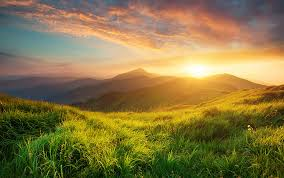
\includegraphics[width=0.4\textwidth]{figures/图文测试/2.jpg} & 日出时分,山间草甸被晨光染成金色,仿佛时间静止。这一刻的宁静,让人忘却尘世喧嚣,只想与这美景共存。 \\
\hline
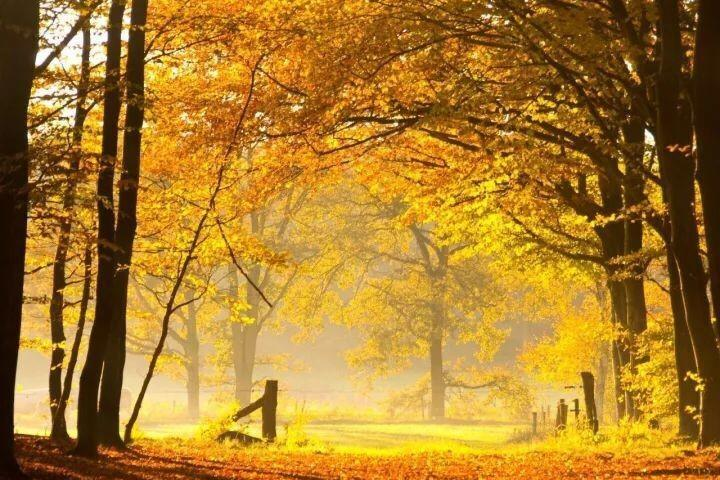
\includegraphics[width=0.4\textwidth]{figures/图文测试/3.jpg} & 落叶铺满的小径,每一步都踏着季节的尾声。阳光透过树梢,却照不进那片即将离去的绿意。感伤的是,这秋日的美景,终究抵不过时间的流逝。 \\
\hline
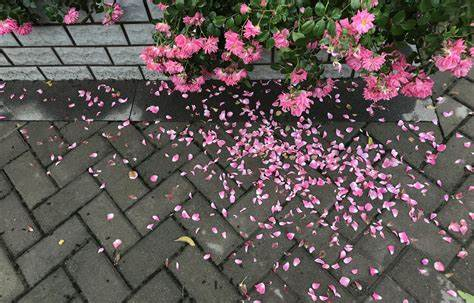
\includegraphics[width=0.4\textwidth]{figures/图文测试/4.jpg} & 落花有意,流水无情,这满地的花瓣,像是春天的泪痕。它们曾是枝头的骄傲,如今却只能随风飘散,让人不禁感叹生命的短暂和无常。 \\
\hline
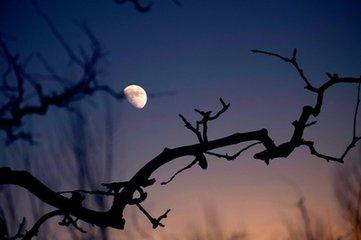
\includegraphics[width=0.4\textwidth]{figures/图文测试/5.jpg} & 月挂枝头,清辉洒落,映照着这孤寂的冬枝。这轮明月,是否也在远方照亮了你的窗前?思念如潮,涌上心头,却只能遥寄于这无声的月色。 \\
\hline
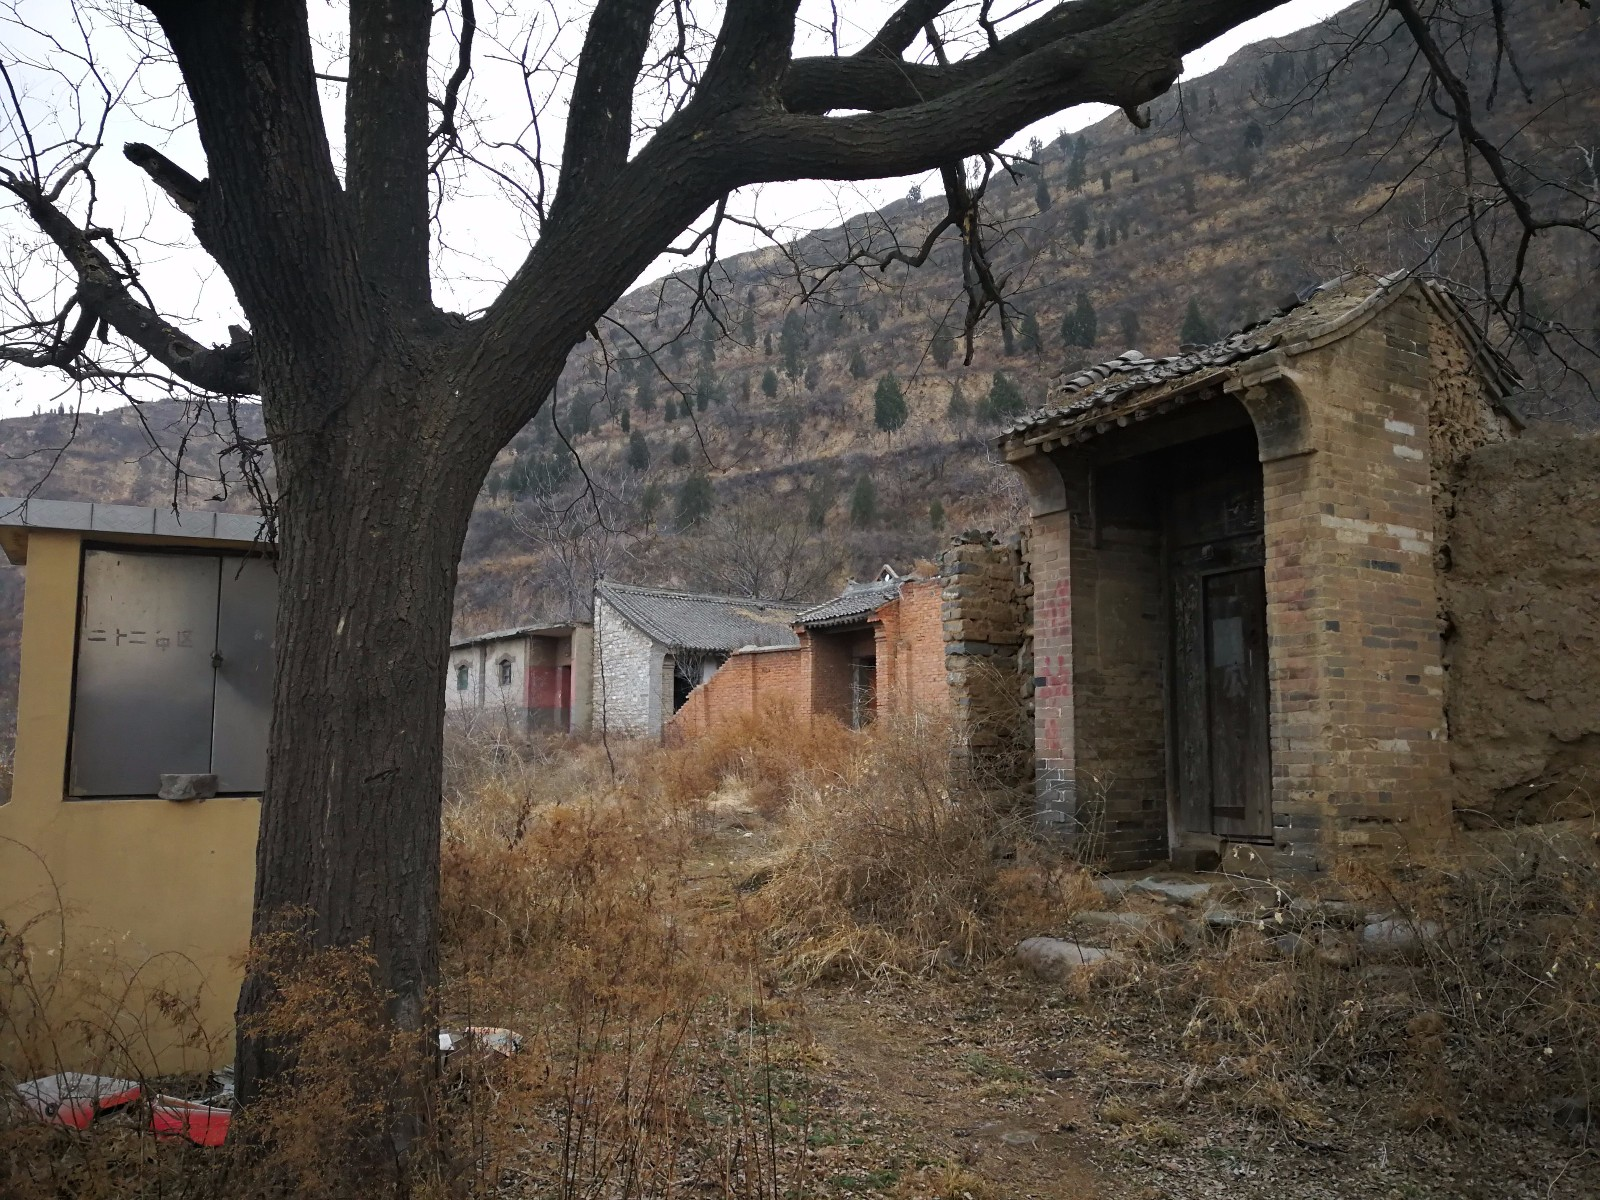
\includegraphics[width=0.4\textwidth]{figures/图文测试/6.jpg} & 老树、旧屋、枯草,时光在这里仿佛凝固。这寂静的村落,承载着多少代人的记忆与故事。我在这里,寻找着那些被岁月遗忘的温馨。 \\
\hline

\end{longtable}


% \begin{table}[ht]
%   \centering
%   \caption{文图古诗生成实验测试集}
%   \label{tab:data_modality_test}
%   \begin{tabularx}{\textwidth}{
%     |>{\centering\arraybackslash}m{0.5\textwidth} % 第一列,居中
%     |>{\centering\arraybackslash}m{0.45\textwidth}|   % 第二列,居中
%     }
%   \hline
%   % \hline
%   图片&文本\\
%   \hline
%   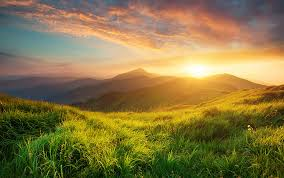
\includegraphics[width=0.5\textwidth]{figures/图文测试/2.jpg} & 日出时分,山间草甸被晨光染成金色,仿佛时间静止。这一刻的宁静,让人忘却尘世喧嚣,只想与这美景共存。 \\
%   \hline
%   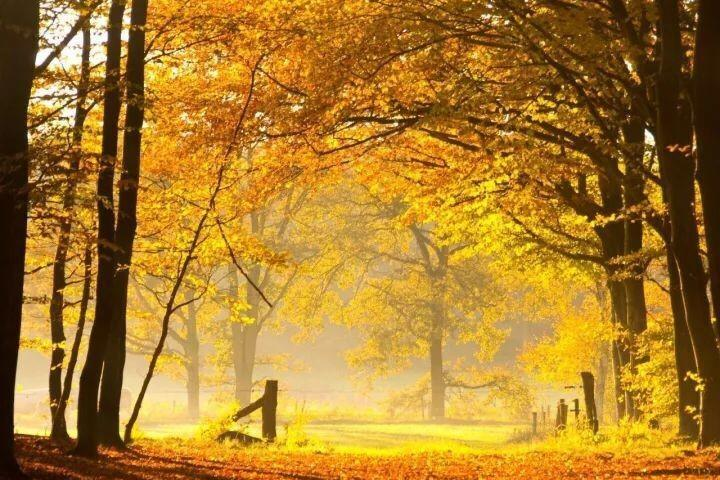
\includegraphics[width=0.5\textwidth]{figures/图文测试/3.jpg} & 落叶铺满的小径,每一步都踏着季节的尾声。阳光透过树梢,却照不进那片即将离去的绿意。感伤的是,这秋日的美景,终究抵不过时间的流逝。 \\
%   \hline
%   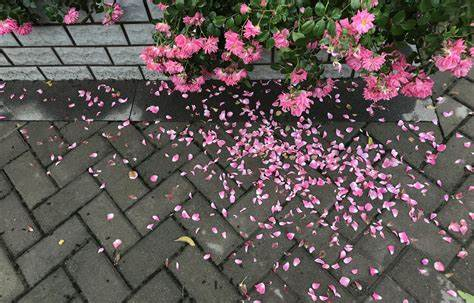
\includegraphics[width=0.5\textwidth]{figures/图文测试/4.jpg} & 落花有意,流水无情,这满地的花瓣,像是春天的泪痕。它们曾是枝头的骄傲,如今却只能随风飘散,让人不禁感叹生命的短暂和无常。 \\
%   \hline
%   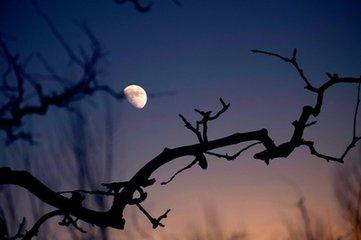
\includegraphics[width=0.5\textwidth]{figures/图文测试/5.jpg} & 月挂枝头,清辉洒落,映照着这孤寂的冬枝。这轮明月,是否也在远方照亮了你的窗前?思念如潮,涌上心头,却只能遥寄于这无声的月色。 \\
%   \hline
%   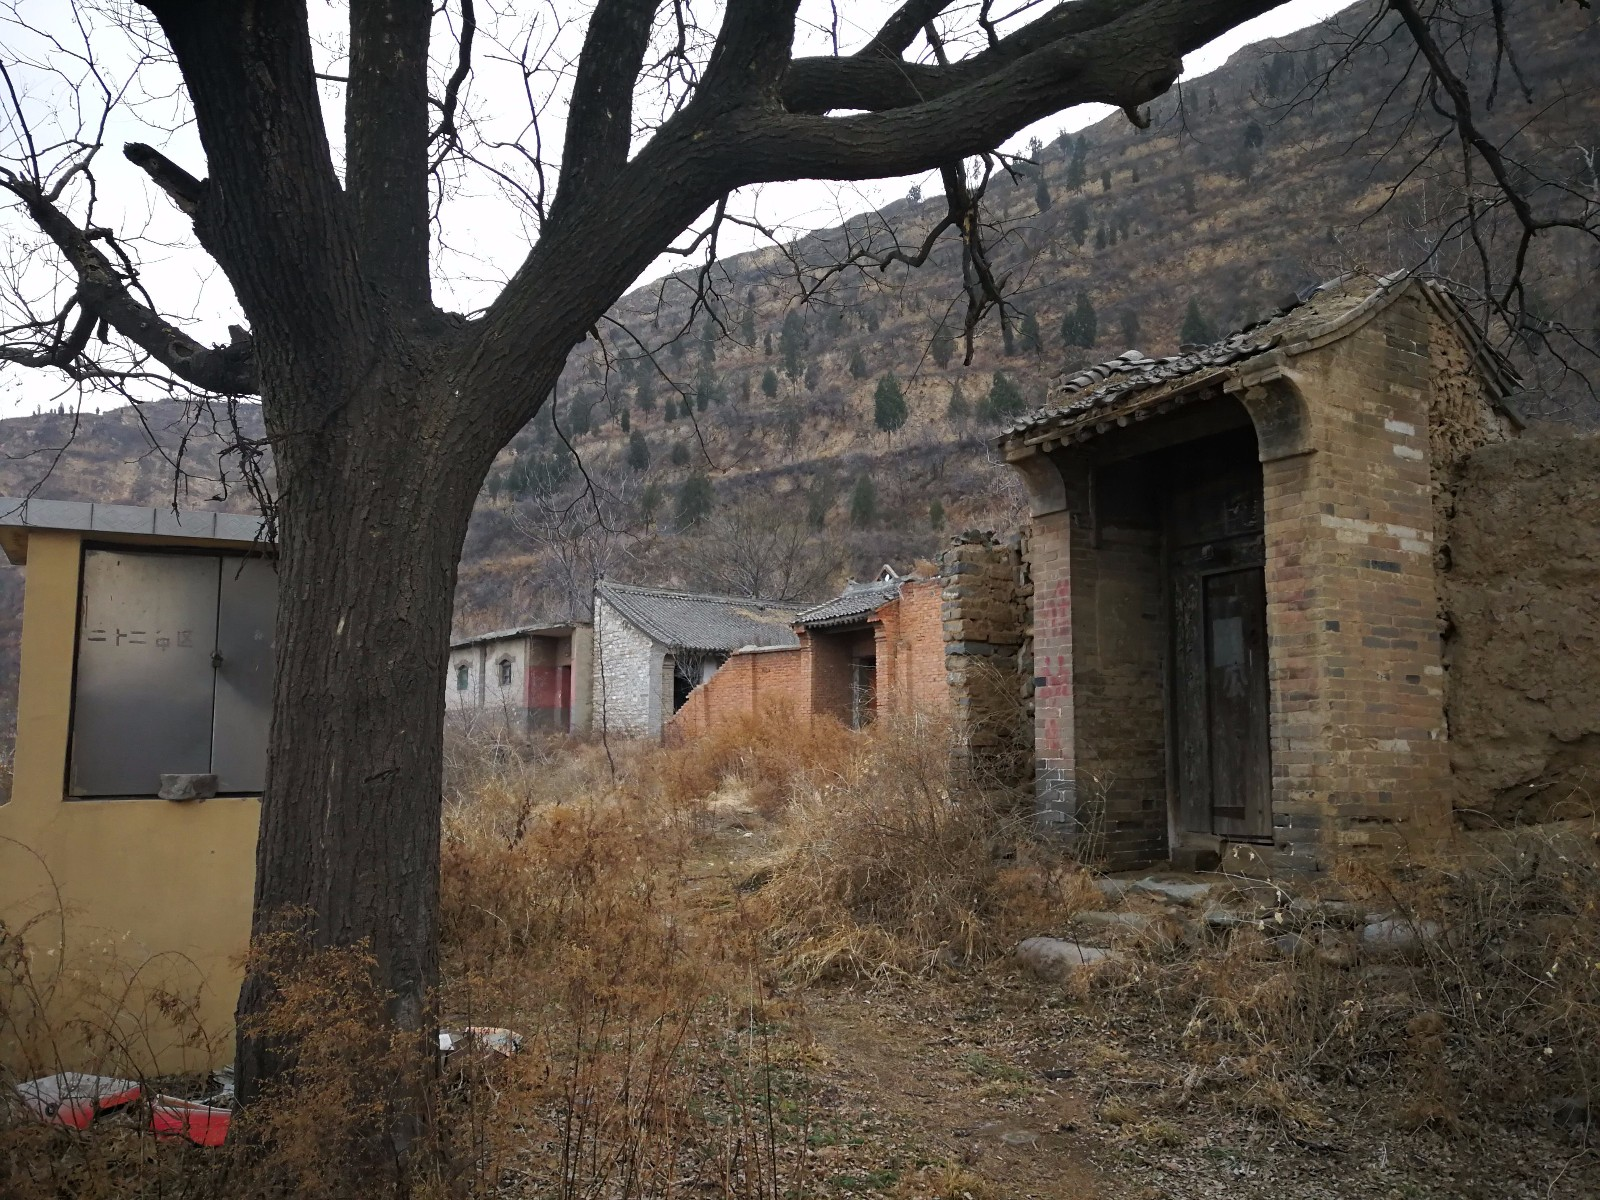
\includegraphics[width=0.5\textwidth]{figures/图文测试/6.jpg} & 老树、旧屋、枯草,时光在这里仿佛凝固。这寂静的村落,承载着多少代人的记忆与故事。我在这里,寻找着那些被岁月遗忘的温馨。 \\
%   \hline
%   % \includegraphics[width=0.4\textwidth]{example-image-b} & 这是图片B的说明文字 \\
%   \end{tabularx}
% \end{table}
  

\clearpage
\section{本章小结}

本章通过一系列实验对系统的古诗生成和评价功能进行了全面验证。实验结果表明,系统在不同方面表现出了一定的优势和局限性。

在古诗生成实验中,基于《唐诗三百首》的白话文翻译输入,ERNIE-4.0和DeepSeek-R1两种模型的输出在BLEU和ROUGE指标上均取得了较高的分数。然而,由于训练数据与测试数据存在重叠,导致实验结果未能有效验证模型的生成能力,无法真实反映模型在独立数据上的表现。

在评分功能实验中,系统对不同质量等级的古诗进行了评分测试。通过分析“诗词中国”传统诗词创作大赛的获奖作品以及经典唐诗和打油诗的评分结果,系统能够较为准确地识别出古诗的质量差异,并在多个维度上给出与真实结果一致的评分,且相较于之前的工作有更好的区分度。这证明了系统评分功能的有效性和可信度。

在自动度量方法的验证方面,BLEU和ROUGE指标在古诗质量评估中表现出了一定的有效性,尤其是在多gram的覆盖度计算上,能够较好地反映古诗的质量差异。然而,BLEU-1指标在某些情况下存在局限性,可能会因简单的一元组覆盖度而误判古诗质量。Similarity指标在语义连贯性方面存在明显局限,其基于词向量模型的计算方法可能会因语法结构对称而误判质量,且本文使用的词向量模型Bert-CCPoem可能不适应这类下游任务,仍有待进一步研究。Distinct指标虽然能够反映用词多样性,但并不能独立地评估古诗的整体质量。

在文图跨模态输入的作用方面,在三种不同的模态组合输入下生成的古诗并未展现出显著的质量差异,这表明DeepSeek-R1的生成能力足以应对不同模态的输入,且在古诗质量上并未受到图像输入的显著影响。然而,图像输入仍然能够帮助用户更好地传达丰富的视觉场景信息,从而提升用户体验。